\documentclass[12pt]{article}
\usepackage{parskip}
\usepackage[letterpaper, margin=1in]{geometry}
\usepackage{graphicx}
\usepackage{amsmath}
\title{ELECENG 2EI5 Lab 1}
\author{Raeed Hassan \\ hassam41 \\  \\ McMaster University}
\renewcommand{\thesection}{\Alph{section}}
\begin{document}
\maketitle
\pagebreak
\section{The Mininmum}
\begin{enumerate}
    \setcounter{enumi}{1}
    \item The resistor used is a 10k resistor. The black wire is ground. The yellow wire is E. The orange wire is V1. The red wire V2.
    \begin{center}
        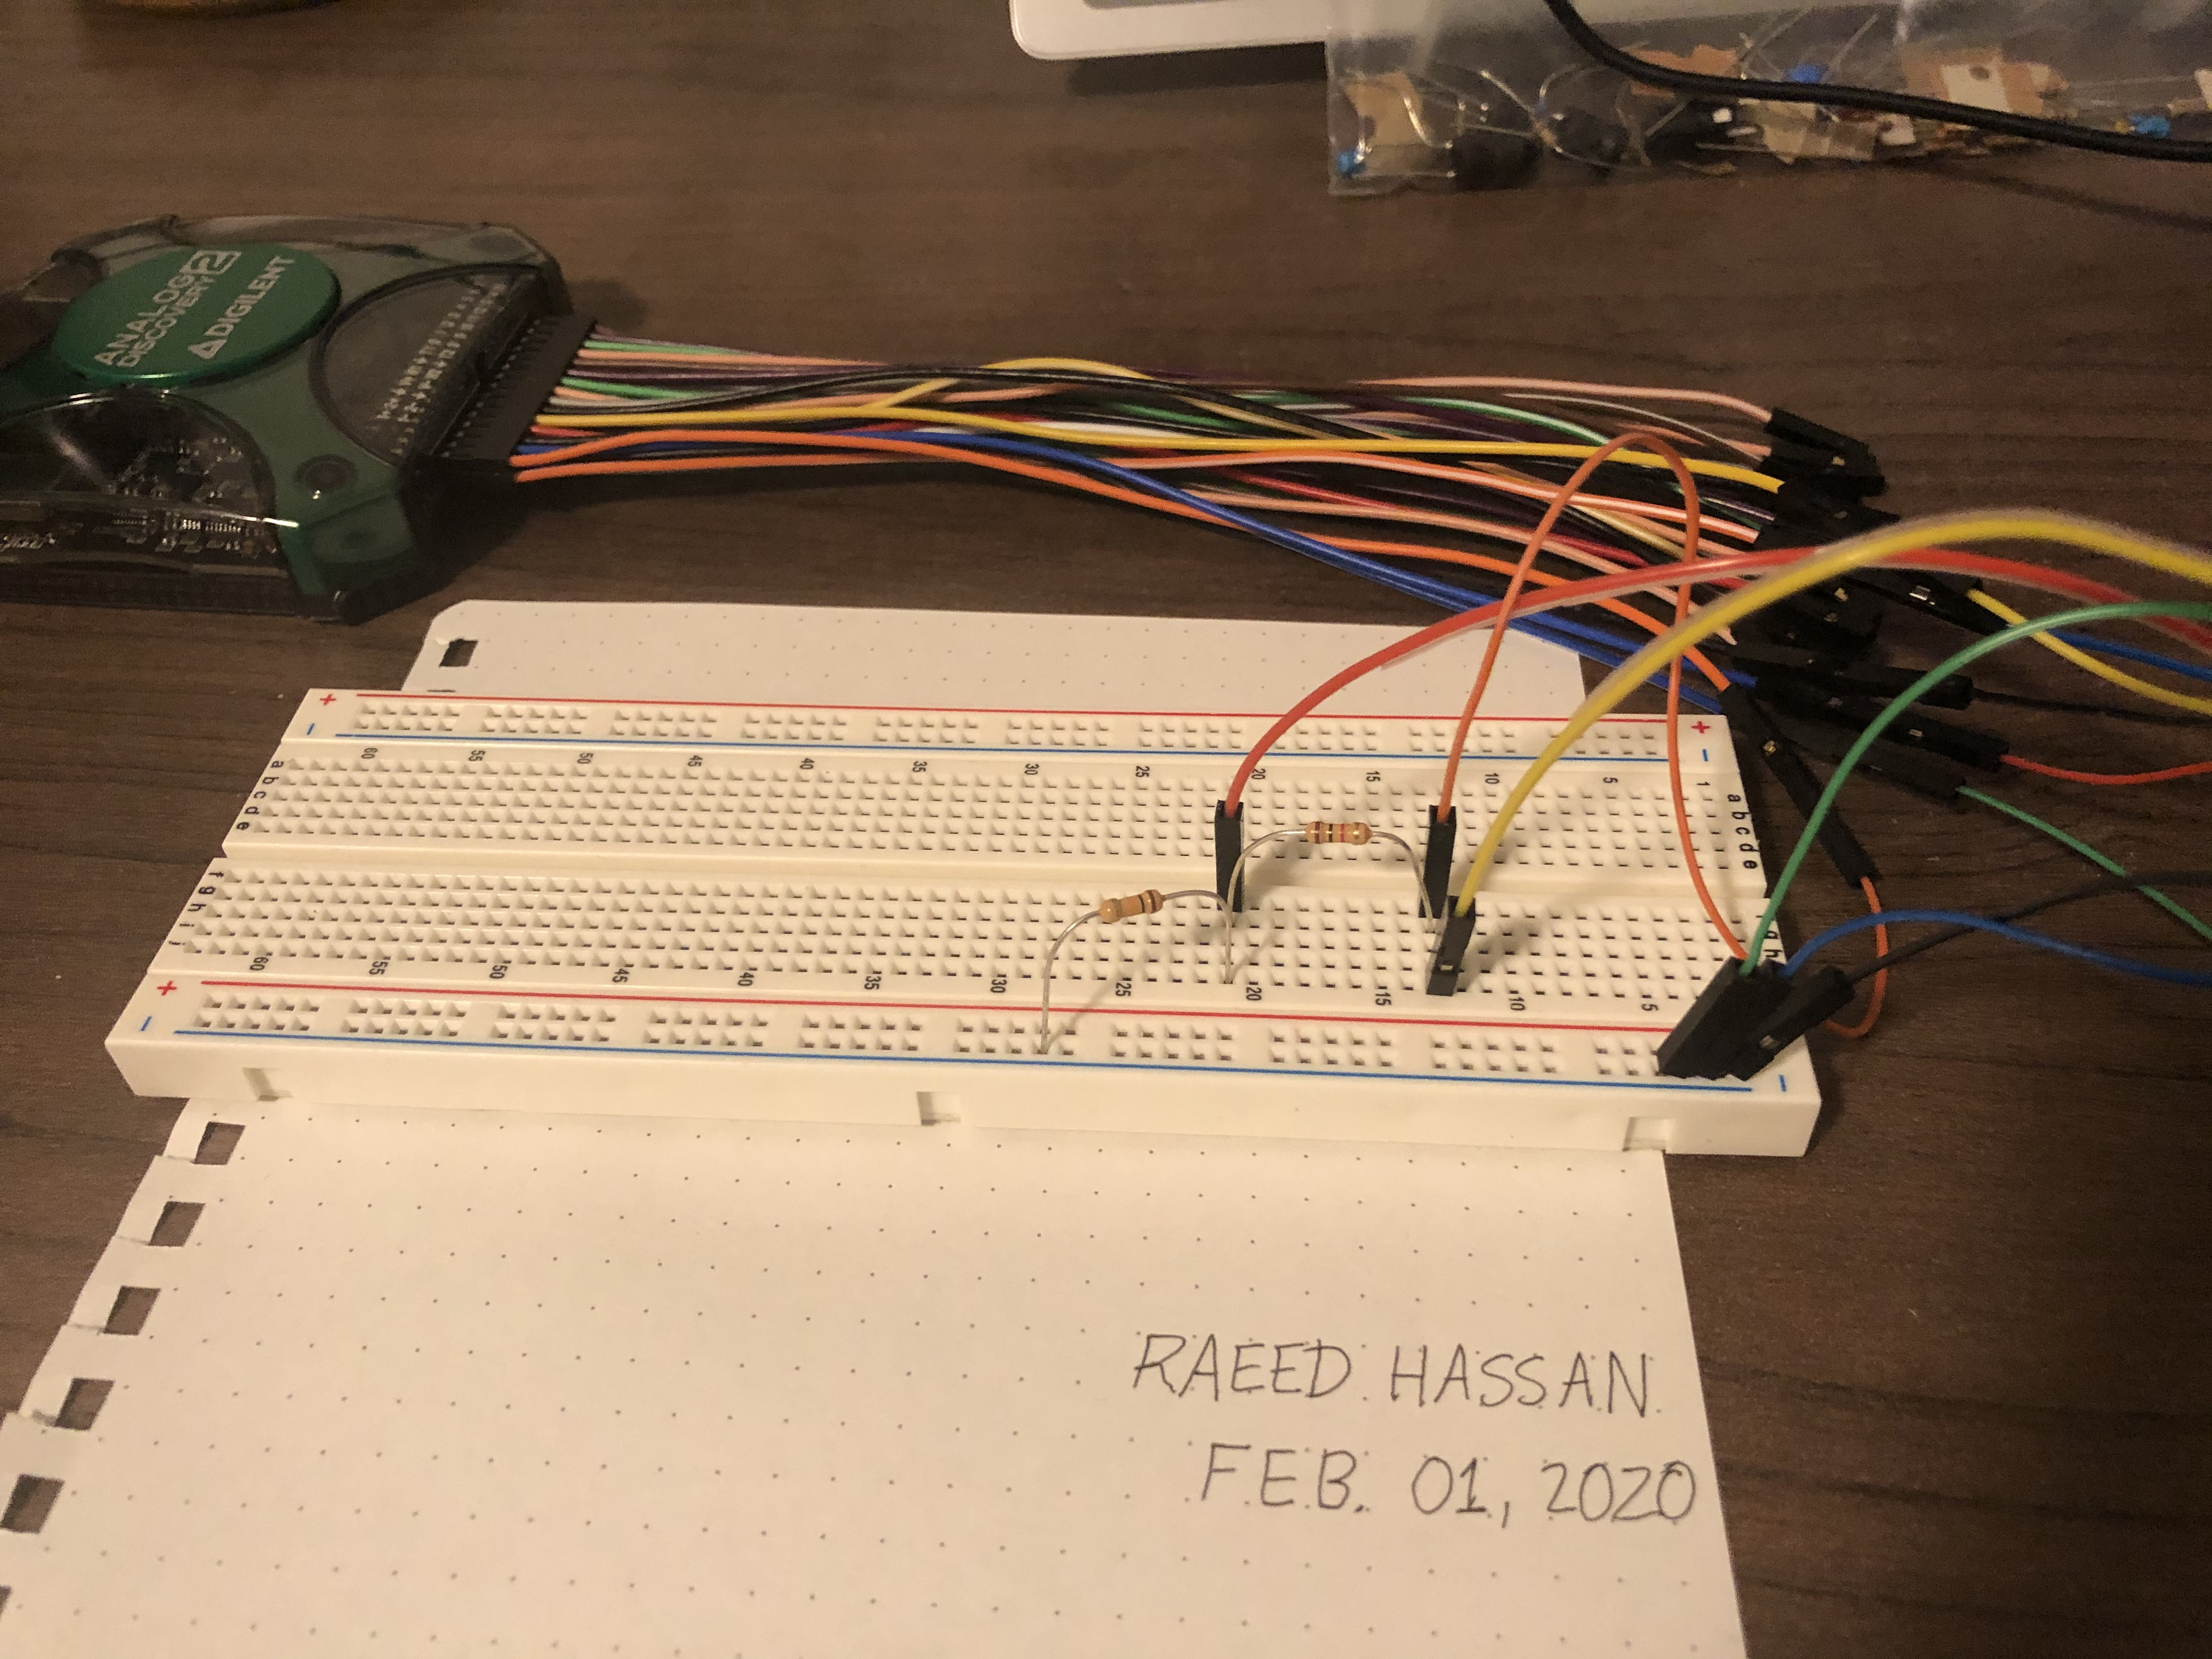
\includegraphics[width=0.82\linewidth]{images/A2.png}
    \end{center}

    \setcounter{enumi}{3}
    \item The horizontal axis is V2 (C2 on scope) and the vertical axis is V1-V2 (M1 on scope).
    \begin{center}
        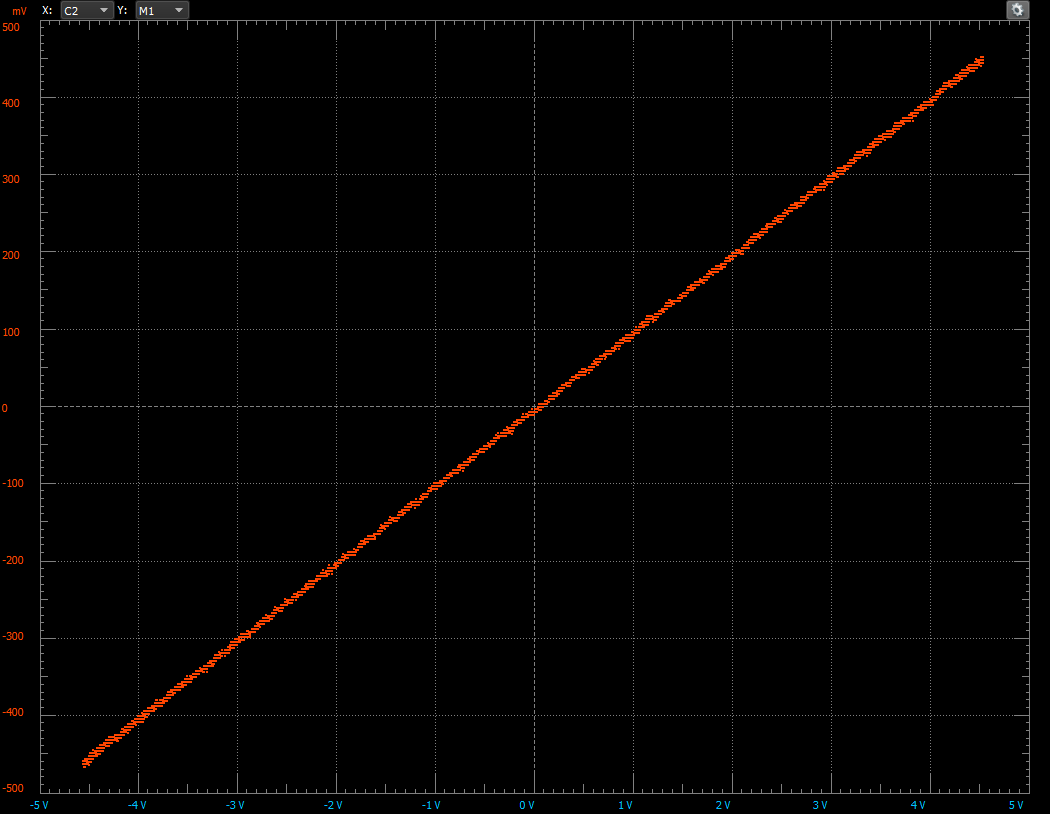
\includegraphics[width=0.82\linewidth]{images/A4.png}
    \end{center}

    \item
    \[
        \begin{aligned}
            V_2 &= \frac{E_1 \cdot R_2}{R_1 + R_2} \\
            E_1 &= V_1 \\
            V_2 &= \frac{V_1 \cdot R_2}{R_1 + R_2} \\
            R_2 &= \frac{V_2 \cdot R_1}{V_1 - V_2} \\
        \end{aligned} 
    \]
    The slope of the plot with $V_2$ on the x-axis and $V_1-V_2$ on the y-axis is $\frac{V_1-V_2}{V_2}$. To determine $R_2$, we need calculate the inverse of the slope of the plot and multiply it by $R_1$. The slope of the plot is approximately 0.099, therefore the value of $R_2 = \frac{1}{0.099} \cdot R_1 = \frac{1}{0.099} \cdot 1000\Omega = 10133\Omega$. The resistor used had a value of 10000$\Omega$ with a tolerance of $\pm$ 5\%. The resistance value calculated for the resistor used as $R_2$ is within the tolerance of the nominal resistance value of the resistor.
\end{enumerate}

\section{The Bulk}
\begin{enumerate}
    \item The horizontal axis is V2 and the vertical axis is V1-V2.
    \begin{center}
        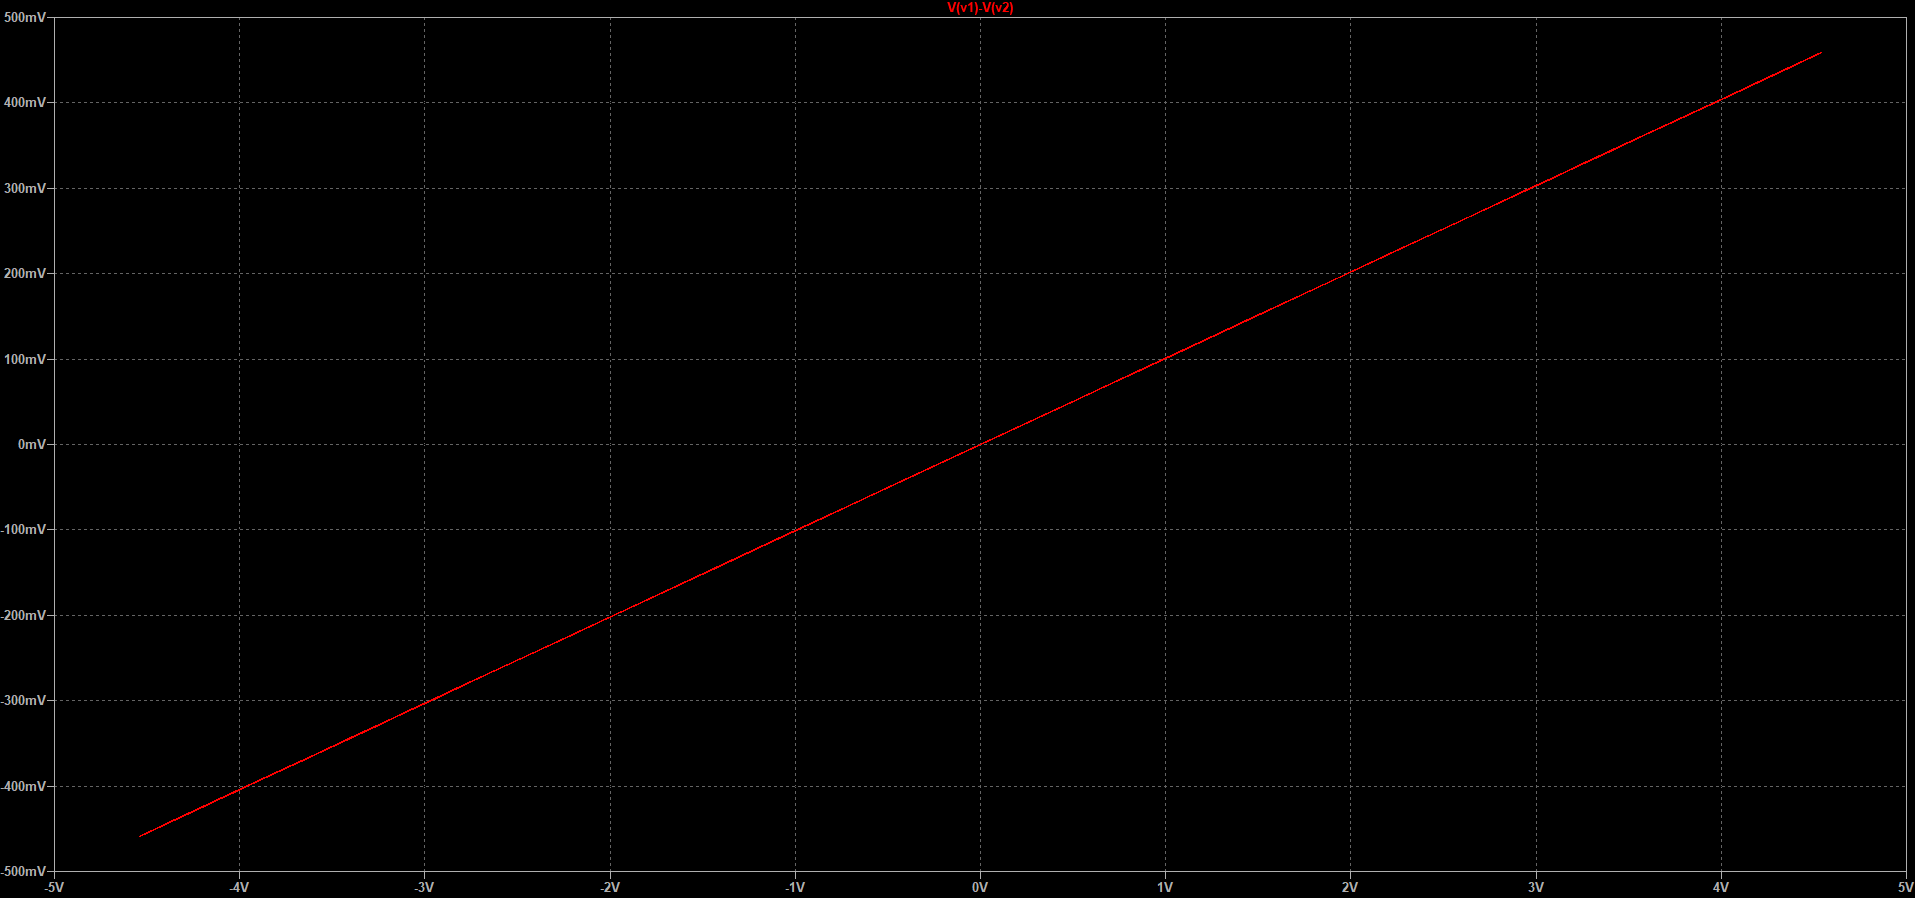
\includegraphics[width=\linewidth]{images/B1.png}
    \end{center}

    \item The experimental plot and the simulated plot follow same shape and have very similar values. Sources of error include resistances of wires, variation in resistance of resistors due to tolerances, internal resistance of voltmeter (an ideal voltmeter has infinite internal resistance), and the calibration of the Analog Discovery 2.
    \pagebreak
    \item Replace R2 with other devices and report the iv-characteristics measured. Choose any three of the following:
    \begin{enumerate}
        \setcounter{enumii}{2}
        \item Capacitor
        \begin{center}
            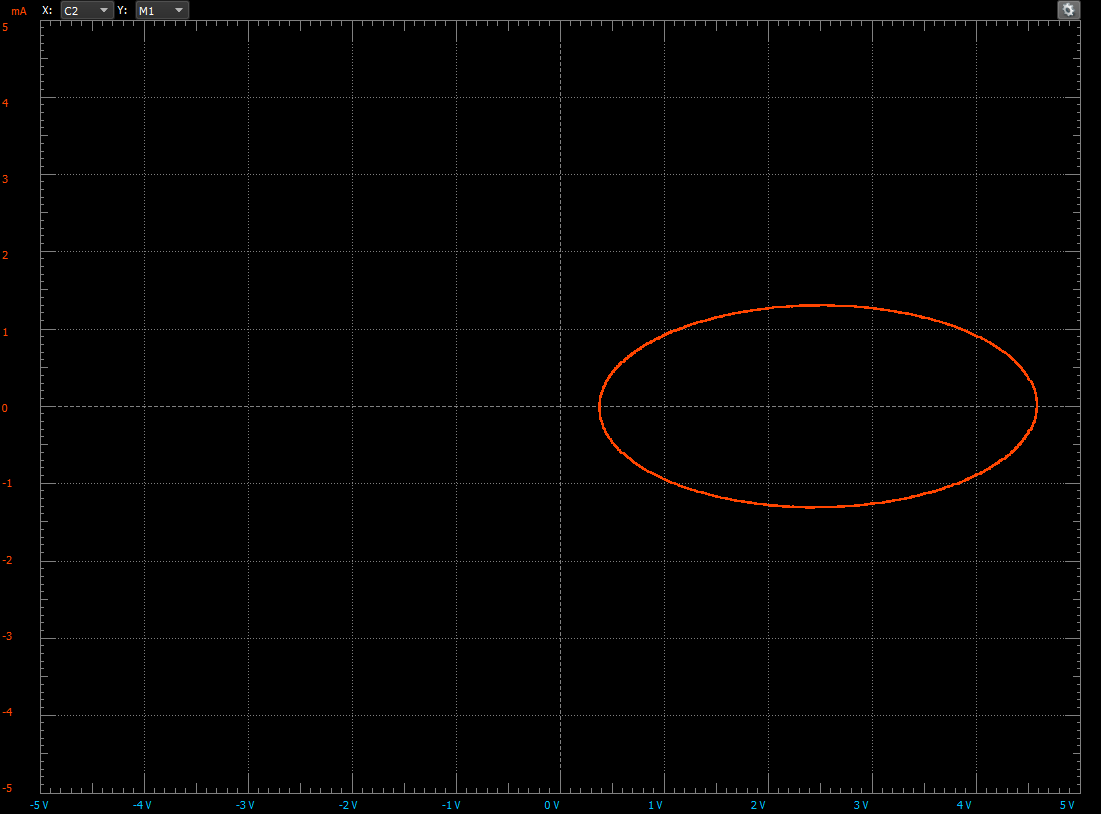
\includegraphics[width=0.97\linewidth]{images/B3c.png}
        \end{center}
        \item 1N4148
        \begin{center}
            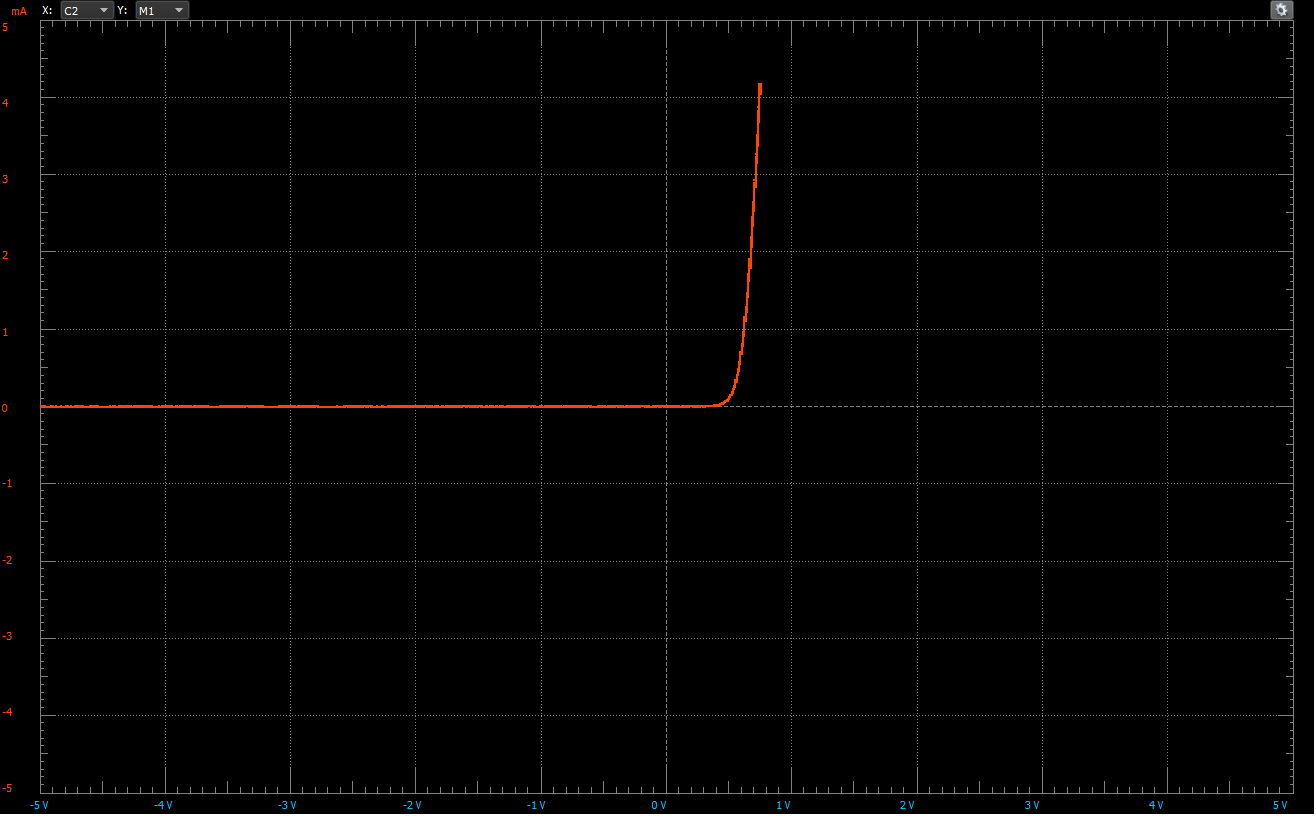
\includegraphics[width=\linewidth]{images/B3d.png}
        \end{center}
        \setcounter{enumii}{5}
        \item LED
        \begin{center}
            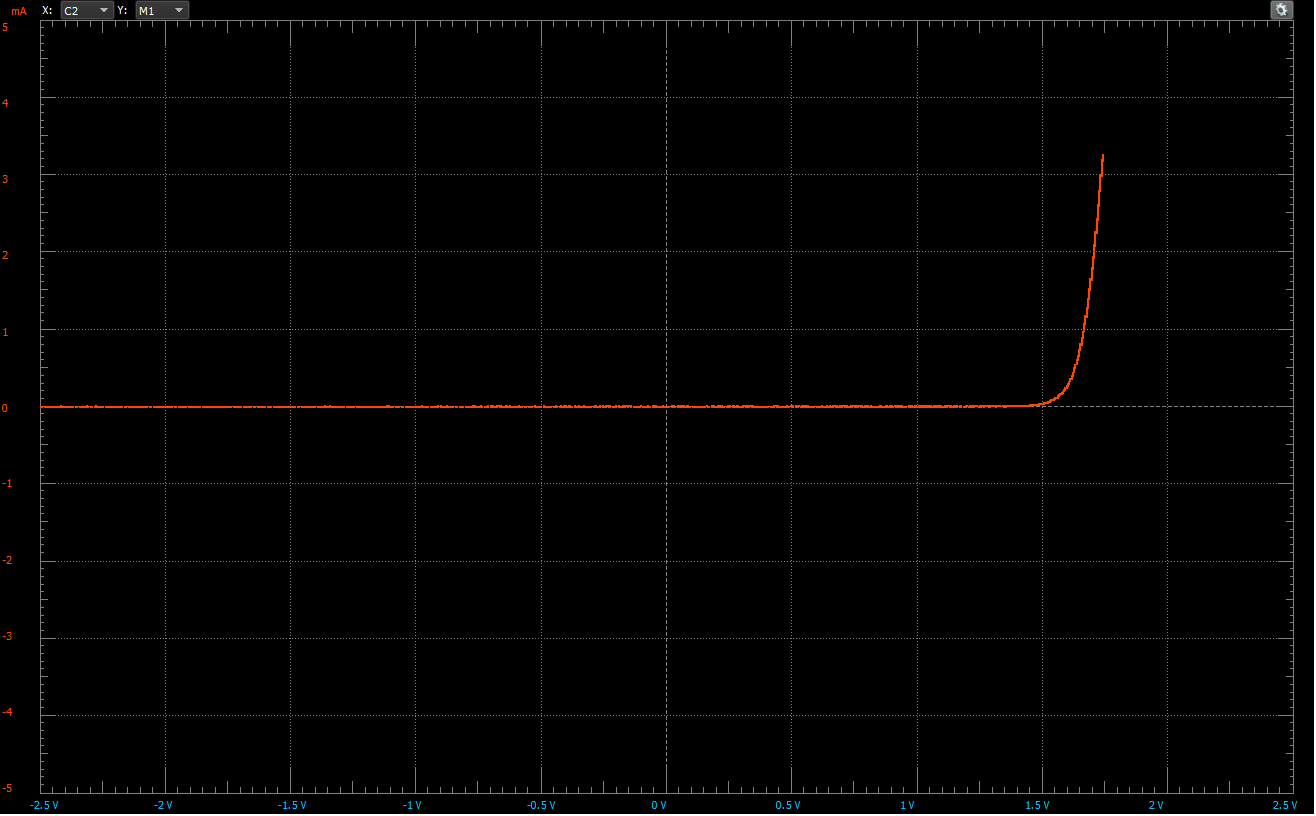
\includegraphics[width=\linewidth]{images/B3f.png}
        \end{center}
    \end{enumerate}
    
    \item Simulate two of the measurements that you did for step 3 above (this cannot include option a).
    \begin{enumerate}
        \setcounter{enumii}{3}
        \item 1N4148 
        \begin{center}
            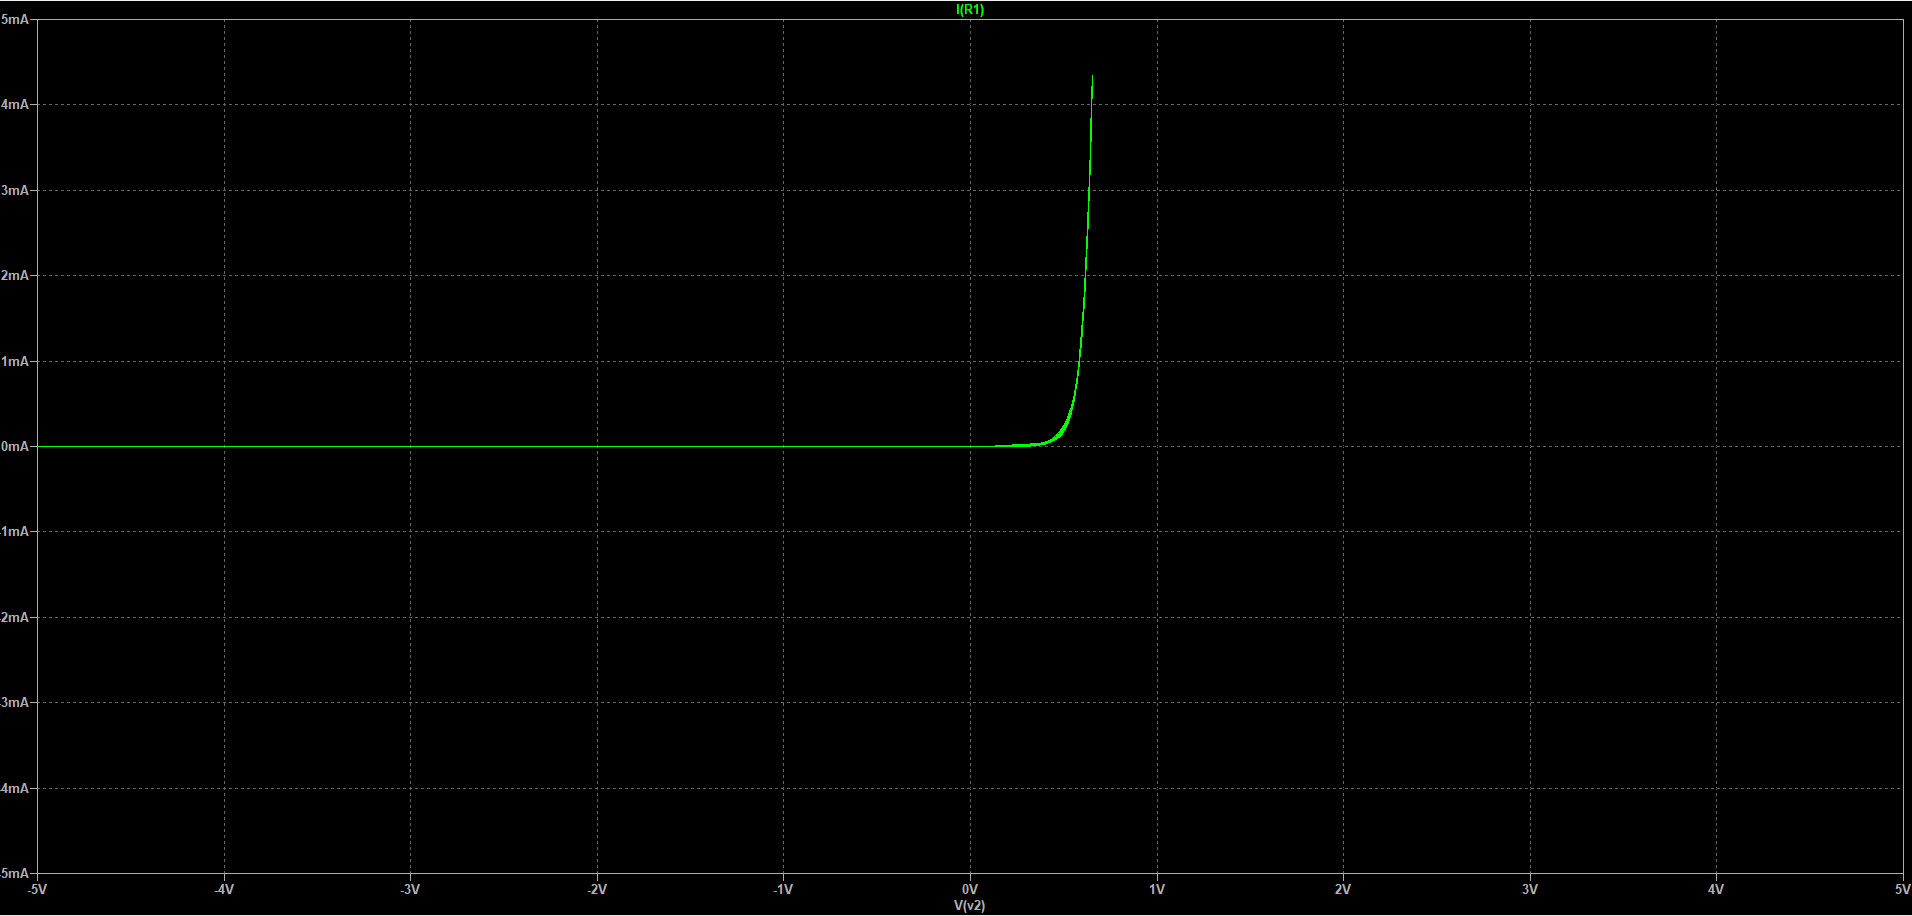
\includegraphics[width=\linewidth]{images/B4d.png}
        \end{center}
        \pagebreak
        \setcounter{enumii}{5}
        \item LED
        \begin{center}
            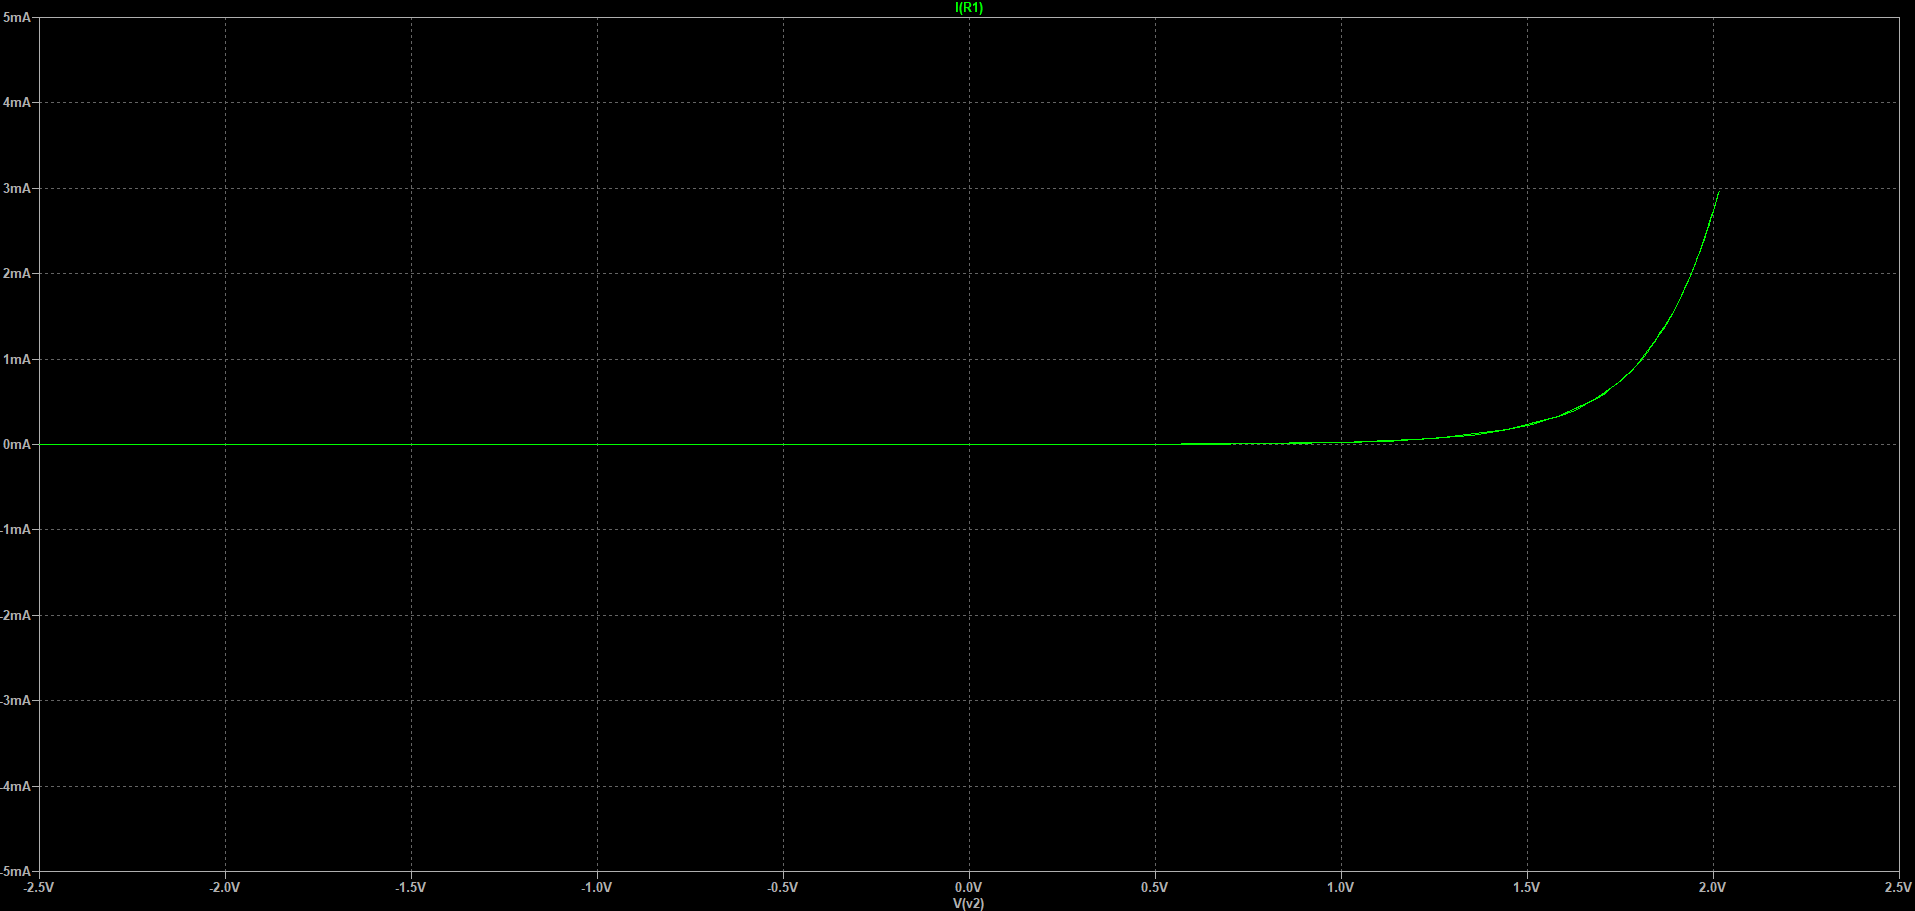
\includegraphics[width=\linewidth]{images/B4f.png}
        \end{center}
    \end{enumerate}
\end{enumerate}

\section{The Max}
A potential problem in measurement from R1 being too small is that it would act like a short circuit and draw too much current from the source, potentially affecting your measurements. A potential problem in measurement from R1 being too large is that it would act like a open circuit and not draw enough current from the source, potentially affecting your measurements.

%\section{The Bonus}
\end{document}